 \documentclass[structabstract]{aa}

\usepackage{natbib}
\usepackage{graphicx}
\usepackage{epstopdf}
\usepackage{color}
\usepackage{hyperref}
\hypersetup{colorlinks, citecolor=blue, filecolor=black, linkcolor=black, urlcolor=black}


\newcommand{\vdag}{(v)^\dagger}
\newcommand{\myemail}{jbyrne@ifa.hawaii.edu}

%%I'm adding these -JPB
%\newcommand{\solphys}{{\it Solar Physics}}
%\newcommand{\aap}{    {\it Astronomy \& Astrophysics}}
%\newcommand{\aaps}{   {\it Astronomy \& Astrophysics Supplemental}}
%\newcommand{\apj}{    {\it Astrophysical Journal}}
%\newcommand{\apjl}{    {\it Astrophysical Journal Letters}}
%\newcommand{\jgr}{    {\it Journal of Geophysical Research}}
%\newcommand{\aapr}{    {\it Astronomy \& Astrophysics Review}}
%\newcommand{\grl}{    {\it Geophysical Research Letters}}
\newcommand{\lrsp}{    {\it Living Rev. Solar Phys.}}
\newcommand{\stat}{Ann. Stat.}

\newcommand{\RNum}[1]{\uppercase\expandafter{\romannumeral #1\relax}}

\usepackage{subfigure}

%\makeatletter
%\newcommand*{\rom}[1]{\expandafter\@slowromancap\romannumeral #1@}
%\makeatother


\begin{document}

\title{Inspecting numerical methods for determining the kinematics of coronal mass ejections and coronal waves}

\titlerunning{Inspecting numerical methods for determining the kinematics of CMEs and coronal waves}
\authorrunning{Byrne et al.}

\author{J.P.~Byrne\inst{1}
	\and D.M.~Long\inst{2}
	\and P.T.~Gallagher\inst{3}
	\and S.A.~Maloney?\inst{4}
	\and S.D.~Bloomfield?\inst{3}
	\and H.~Morgan\inst{5,1}
	\and S.R.~Habbal\inst{1}}
\institute{Institute for Astronomy, University of Hawai'i, 2680 Woodlawn Drive, Honolulu, HI 96822, USA.\\
		\email{jbyrne@ifa.hawaii.edu}
		\and
		UCL--Mullard Space  Science Laboratory, Holmbury St. Mary, Dorking, Surrey, RH5 6NT, UK.
		\and 
		School of Physics, Trinity College Dublin, College Green, Dublin 2, Ireland.
		\and
		Skytek, 51/52 Fitzwilliam Square West, Dublin 2, Ireland
		\and
		Institute of Mathematics and Physics, Aberystwyth University, Ceredigion, SY23 3BZ, UK.
		}

\date{Received ?; accepted ?}
%%Abstract
\abstract
% Context (optional)
{\emph{Why are we doing this work?} }
% Aims (mandatory)
{In this paper we show that traditional techniques for the determination of CME and ``EIT wave'' kinematics, as currently applied, do not return accurate estimates of the true kinematics of the feature. We highlight the errors inherent in these approaches and illustrate a recipe for accurate estimates of the kinematics using a residual resampling bootstrapping approach to determine the confidence interval associated with the model used to measure them.}
% Methods (mandatory)
{We discuss the errors inherent in the use of numerical differentiation techniques when applied to small data--sets. We present a residual resampling bootstrapping approach as a statistically rigorous technique for the determination of accurate kinematic estimates.}
% Results (mandatory)
{It is shown that accurate feature kinematics can only be estimated by applying a pre--determined model to the position measurements. The validity of this model must be based on the physical properties of the feature that are to be measured, and the accuracy of applying that model to the data can be examined using a bootstrapping approach to determine the confidence interval associated with the estimated model parameters.}
% Conclusions (optional)
{\emph{What are our conclusions?}}

%% Keywords 

\keywords{Sun: activity -- Sun: corona -- Sun: coronal mass ejections (CMEs)}

\maketitle

%
%________________________________________________________________

\section{Introduction}
\label{sect_intro}

% Set the scene
The most defining feature of a transient solar phenomenon such as a Coronal Mass Ejection (CME) or a coronal wave (commonly called an ``EIT Wave'') is its motion. These generally short--lived features, resulting from a solar eruption, are observed to propagate across the solar corona (i.e., coronal waves) or in the case of CMEs, outward from the Sun into the heliosphere. 
Observational catalogues of both phenomena have been compiled over more than $\sim$20~years of observations \citep[e.g.,][]{1985JGR....90..275I,2004JGRA..10907105Y,2009ApJS..183..225T}, with the physical properties of both phenomena very well characterised \citep[see the recent reviews by e.g., ][]{2011SSRv..158..365G,2012SoPh..tmp...93P,2011ASSL..376.....H,2012LRSP....9....3W}. 

% We're interested in motion here
As transient phenomena, the kinematics of both sets of features continue to be one of the most important characteristics used to classify them. The motion of both phenomena is traditionally identified using difference images, where a preceding image is subtracted from a leading image to highlight motion, allowing the feature to be identified ``by eye''. However, this approach highlights \emph{relative} rather than \emph{actual} motion, and is prone to undefined user--dependent bias. More recent work has used single image processing techniques such as wavelet transforms \citep{2009A&A...495..325B,2012ApJ...752..144M} and automated approaches \citep[e.g.,][]{2011A&A...531A..42L,2012ApJ...752..145B,2012SoPh..276..479P} to minimise user--error and reveal the true physical characteristics of the feature. By tracking the position of the feature with time it is possible to determine its kinematics, allowing an insight into the physical properties of the phenomenon. 

% Why we care about kinematics
The kinematics of these features are important for a variety of reasons. The true physical nature of coronal waves is not fully understood, with two main competing theories; that they are waves \citep[e.g.,][]{2012ApJ...754....7S,2010ApJ...716L..57V} or signatures of magnetic field restructuring during a CME eruption \citep[e.g.,][]{2011ApJ...738..167S,2011ApJ...732L..20C}. The kinematics of the feature have been proposed as one of the main discriminators between these competing theories, with the relatively high velocities measured thus far for this phenomenon suggesting a wave interpretation may be appropriate \citep[cf.][]{2011A&A...532A.151W,2012ApJ...753..112Z}. Similarly, CME kinematics are vitally important from a space weather point of view as they allow increased accuracy in the predicted arrival time of the feature at Earth. The kinematic behaviour of the CME very low down in the solar corona may also be used to discriminate between eruption mechanisms \citep[cf.][]{2010A&A...516A..44L}. However \citet{2007ApJ...657.1117W} demonstrate that the errors in CME acceleration values can be of the same order as the accelerations typically measured. 

% The step from distance-time to kinematics
A variety of different mathematical techniques exist for deriving the kinematics of transient features, ranging from the fitting of polynomial functions to the distance--time measurements to the numerical differentiation of the measurements. While these techniques may be mathematically sound, some of them are not necessarily applicable to the derivation of kinematics for these features and can produce spurious results. 


\section{Numerical Differentiation \& Error Propagation (recap)}
\label{sect:num_diff_errors}

When presented with a moving object through a sequence of image frames such that it is possible to measure its position at each time step, the technique of numerical differentiation is often used to derive the velocity and acceleration of the object. In the standard 2-point approach, it should be possible to derive the time evolution of a system at time step $t+\delta t$ according to the system values at time step $t$. This may be applied through the technique of forward, reverse or centre differencing, resulting in an estimate of the speed of the object at a specific time step given its positional information. More commonly, a 3-point Lagrangian interpolation is applied to better approximate the kinematics of a moving object by solving for the Lagrange polynomials that best fit across three given datapoints (e.g. \textsc{deriv.pro} in IDL). Each of these schemes is based upon the Taylor series expansion of a real function $f(t)$:
\begin{equation}
\label{taylor1}
f(t_0+\delta t) \; = \; f(t_0)+f'(t_0)\delta t +  \frac{f''(t_0)}{2!}(\delta t)^{2}  + ...
\end{equation}
but due to the approximation of an infinite series with a finite number of terms and iterations, an error must be associated with the result, based on its deviation from the true solution. Generally the Euler method is employed, using the formula:
\begin{equation}
y_{n+1} \; = \; y_n + h f(t_n, y_n)
\end{equation}
to solve the initial value problem $y'=f(t,y)$ given $y(t_0)=y_0$, where $h$ is the stepsize such that $t_n=t_0+nh$. The convergence of such an approximation to the actual solution is prone to two sources of error; truncation error (the difference between the true solution and the approximation) and round-off error (the limited precision of the approximation). Added to this is the fact that the data measurements themselves are subject to uncertainties in both the positional and temporal information, and the ability of the numerical differentiation techniques to derive kinematics becomes highly jeopardised, as shall be shown.

Given a function $x=f(u,\,v)$, the error propagation equation (based on the standard deviations $\sigma$ of the variables) is written:
\begin{equation}
\label{eqn_errorprop}
\sigma_x^2 \; = \; \sigma_u^2 \left(\frac{\partial x}{\partial u}\right) ^2 + \sigma_v^2 \left( \frac{\partial x}{\partial v} \right) ^2 + 2 \sigma_{uv}^2 \left( \frac{\partial x}{\partial u} \right) \left( \frac{\partial x}{\partial v} \right) + ...
\end{equation}
Specifically in the case of kinematic analyses, this is used to propagate the errors on the distance-time data $r(t)$ into the velocity $v(t)$ and acceleration $a(t)$ profiles to determine the associated uncertainties. In the case of distance-time data the covariance terms are zero because the quantities are uncorrelated.

When presented with relatively low sampling of the data, as in the case of coronagraph observations of CMEs and disk observations of waves, it is generally found that the simplest differentiation techniques are not applicable. The forward and/or reverse differencing techniques act to shift the kinematic profiles by one time-step, which is substantial enough to be of concern here (i.e., they derive a result at the current time-step, based on the pro-/preceding time-step). Centre differencing employs the two neighbouring data-points of the point under examination, and so is a better indication of the result at that time-step, but it fails at both endpoints. In any case these should not be employed when the spacing of the data-points is unequal, i.e., when the cadence $\delta t$ is not constant, and so the 3-point Lagrangian interpolation technique is used (which gives the same result as the centre-difference otherwise, but includes the endpoints and has an associated error propagation formulation). The Lagrangian interpolation polynomial is given by:
\begin{eqnarray}
L(x) \; &=\; \sum_{j=0}^2 y_j l_j(x) \\ \quad \mbox{where} \quad
l_j(x) \; &=\; \prod_{i=0, i\neq j}^2 \frac{x-x_i}{x_j-x_i} 
\end{eqnarray}
The derivative at point $x$ is given by $L'=\partial_x L(x)$. So for the case of height-time data being used to derive velocity (and similarly acceleration) the associated error is given by:
\begin{equation}
\sigma_{v_1}^2 \,=\, \frac{\sigma_{r(t_2)}^2+\sigma_{r(t_0)}^2}{(t_2-t_0)^2} + v^2 \left( \frac{\sigma_{t_2}^2+\sigma_{t_0}^2}{(t_2-t_0)^2} \right)
\label{vel_err}
\end{equation}
as in \textsc{derivsig.pro} in IDL. The endpoint errors are derived from a weighting of the pro/preceding two data--points, that is therefore larger to reflect the unknown nature of the trend beyond the sample points.

Although the 3-point Lagrangian is mathematically sound, its application to solar eruptive event kinematics proves problematic. The main drawbacks are two-fold:
\begin{enumerate}
\item The noise level, especially across low-cadence sampling, can scatters the measurements to such a degree that the numerical derivatives become untrustworthy and even misleading compared to the actual trends of the kinematic data.
\item The error-propagation formulation results in a misleading uncertainty interval on the velocity and acceleration profiles. For example, it counter-intuitively increases for increasing cadence measurements.
\end{enumerate}

Simulations of the drawbacks of a standard numerical derivative are presented in Section~\ref{sect:simul1}. In Section~\ref{sect:simul2} we outline a more appropriate method for inspecting the  kinematics of CMEs and waves, as applied to model data. In Section~\ref{sect:case_studies} some real-data cases are revisited with these methods, and motivate the proposed treatment of data from the new coronal image processing CME catalogue \citep[CORIMP;][]{2012ApJ...752..144M, 2012ApJ...752..145B}, and coronal pulse identification and tracking algorithm catalogue \citep[CorPITA;][]{2011A&A...531A..42L}. A final discussion and conclusions are presented in Section~\ref{sect:conclusions}.


\begin{figure*}
\centering
\subfigure{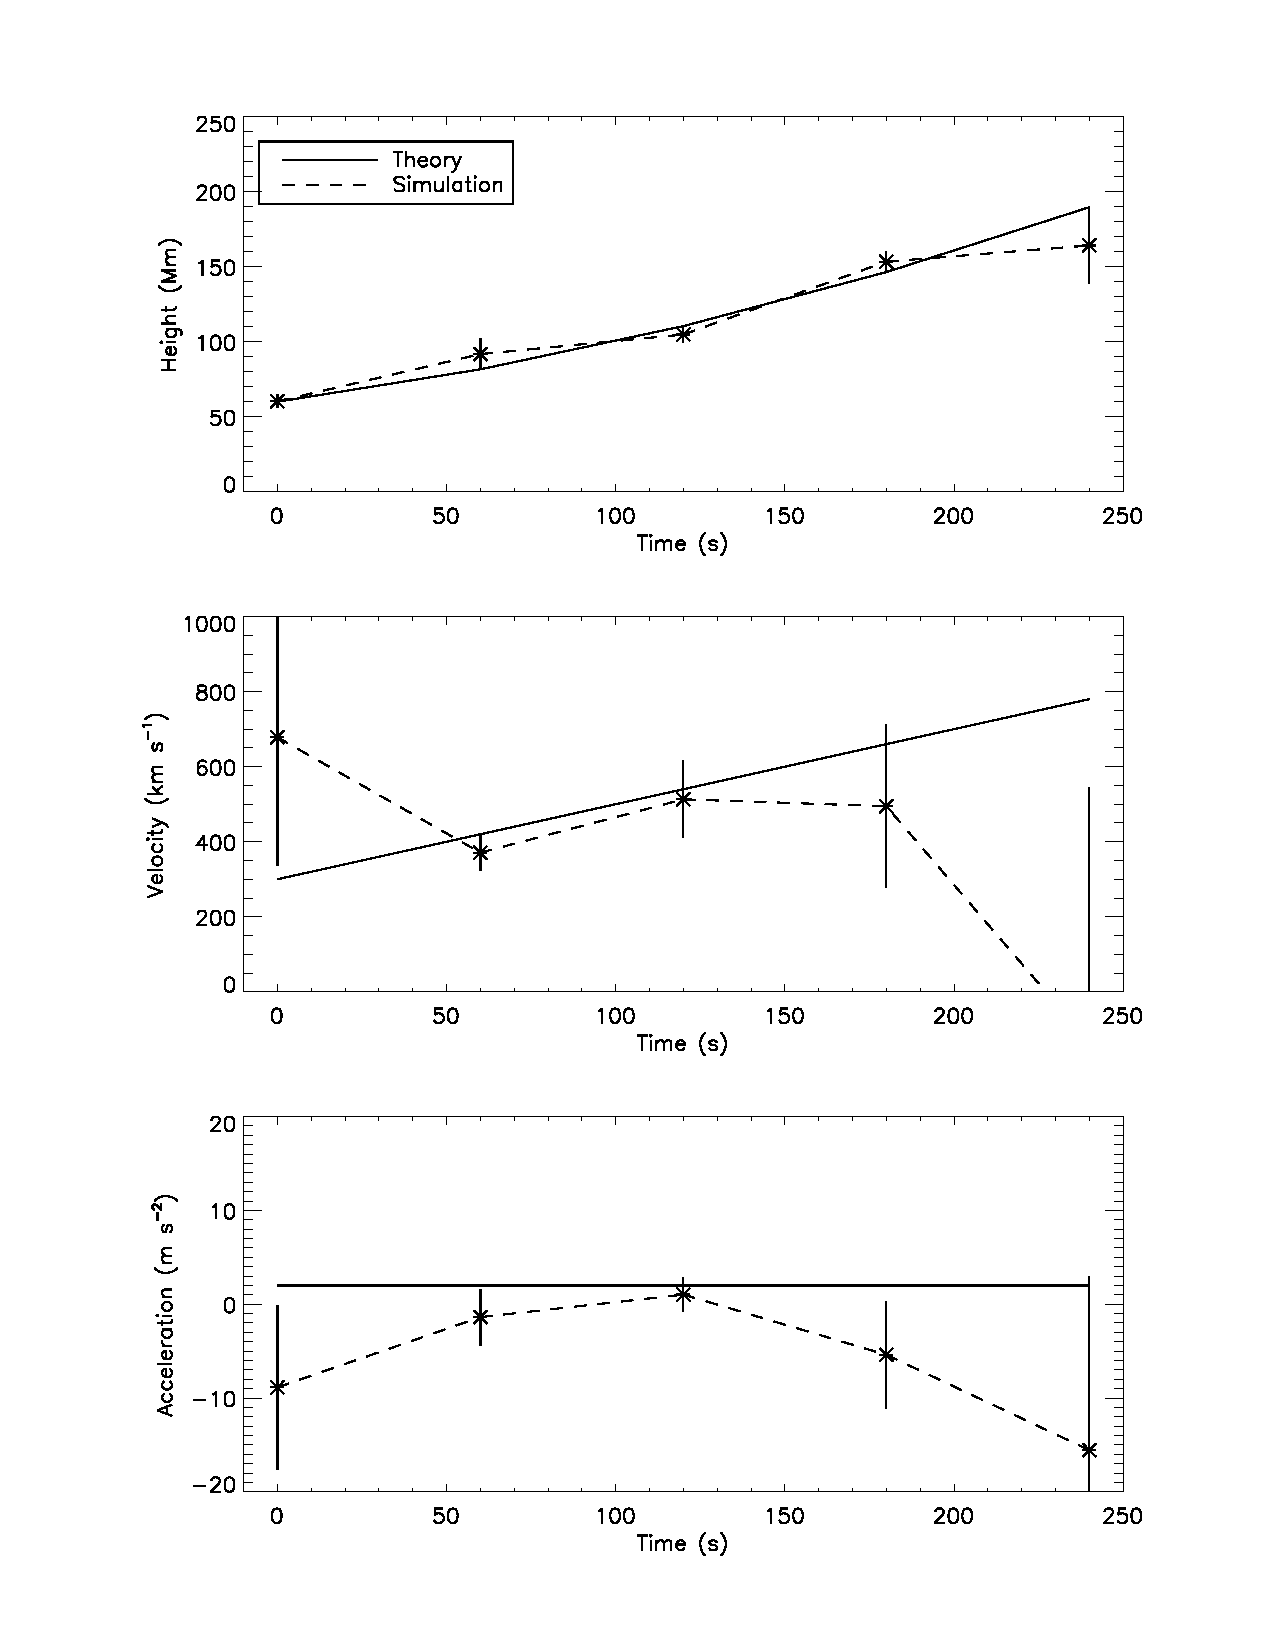
\includegraphics[scale=0.43, trim=110 50 70 70]{images/sim_vels_thesis1.pdf}}
\subfigure{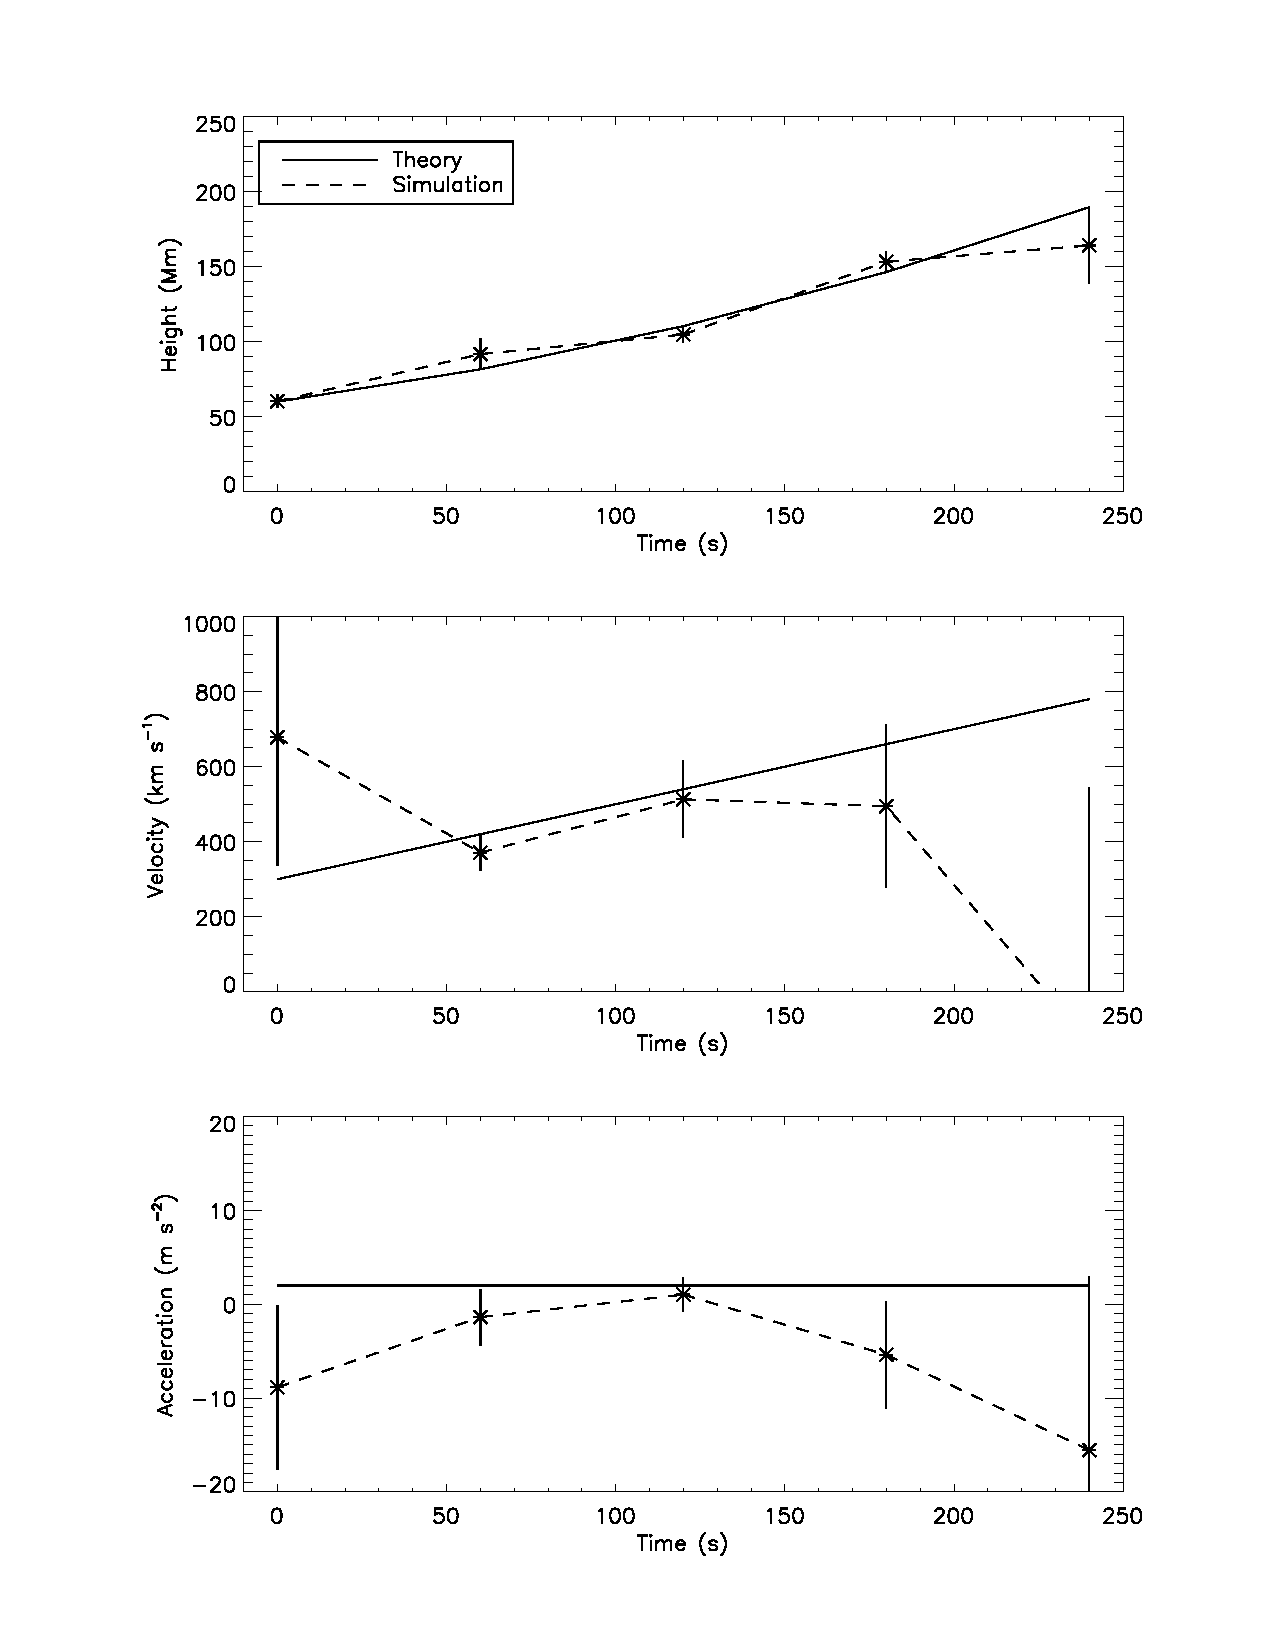
\includegraphics[scale=0.43, trim=70 50 110 70]{images/sim_vels_thesis2.pdf}}
\caption{A theoretical model for a CME with constant acceleration 2\,m\,s$^{-2}$ and initial velocity 300\,km\,s$^{-1}$, and two simulations of how the resulting profiles for a noisy sample of data--points behave using 3-point Lagrangian interpolation.}
\label{sim_vels_thesis}
\end{figure*}

\section{Simulations}
\label{sect:simul1}

In the case of CMEs and waves, there is great motivation to resolve the dynamics of their propagation as precisely as possible in order to study the forces at play. For example, CMEs in general may be undergoing continued driving (internal) forces, or positive or negative drag (external) forces, or most assuredly some interplay of both. Similarly wave propagation may be affected by changes to the low-coronal environment, e.g., low-density coronal hole regions, or strong magnetic field active regions. Thus any changes to event acceleration that result from different phases of dominating force, and where or why this can occur, are of great interest. But the true kinematics of such events remains somewhat elusive given the inherent limitations of the data and the numerical methods employed. In our treatment of both phenomena here, we use cases of simulated CME and wave data interchangeably, to demonstrate both constant and non-constant acceleration profiles with varying scatter and cadence.


\subsection{Effect of noisy scatter on deriving kinematics}
\label{subsect:test_lagrange_const}


As an example of the effect of scatter due to noisy data, we first simulate a simple height-time profile of a CME that propagates according to the quadratic equation:
\begin{equation}
\label{eqn:const_a}
r(t) = r_0 + v_0 t + \frac{1}{2}a t^2
\end{equation}
where $r_0$\,=\,60\,Mm is the initial height, $v_0$\,=\,300\,km\,s$^{-1}$ is the initial velocity, and $a$\,=\,2\,m\,s$^{-2}$ is the acceleration of the CME. Varying levels of noise are randomly added up to a maximum of 20\,\%. An `extreme case' errorbar on each datapoint is determined by its distance from the true height-time profile, to represent a scenario wherein all measurement uncertainties just manage to overlap the true profile. Various instances of randomized datapoint scatters result in erroneous trends in the velocity and acceleration profiles, even with the proper error treatment ascribed by the 3-point Lagrangian interpolation technique, and even in this simplest case of constant acceleration. Two examples are shown in the left and right of Figure~\ref{sim_vels_thesis} where completely opposing acceleration trends are determined for different samplings of the same dataset, indicating that the nature of the scatter in the samples is not satisfactorily reflected in the derived kinematics and their associated errors. At the very least the datapoints should be expected to overlap the truth in each plot so that it remains a valid solution. A possible assurance, even in the case of low-cadence samplings (or very fast events), is that instead of trusting the endpoints they simply be removed. Figure~\ref{sim_vels_thesis} would then show three datapoints for velocity and one datapoint for acceleration, that would go somewhat toward removing the biased trends and imply a constant acceleration close to the true value. However, when dealing with low-number samples especially, it would be better not to have to remove datapoints.

\begin{figure}[t]
\begin{center}
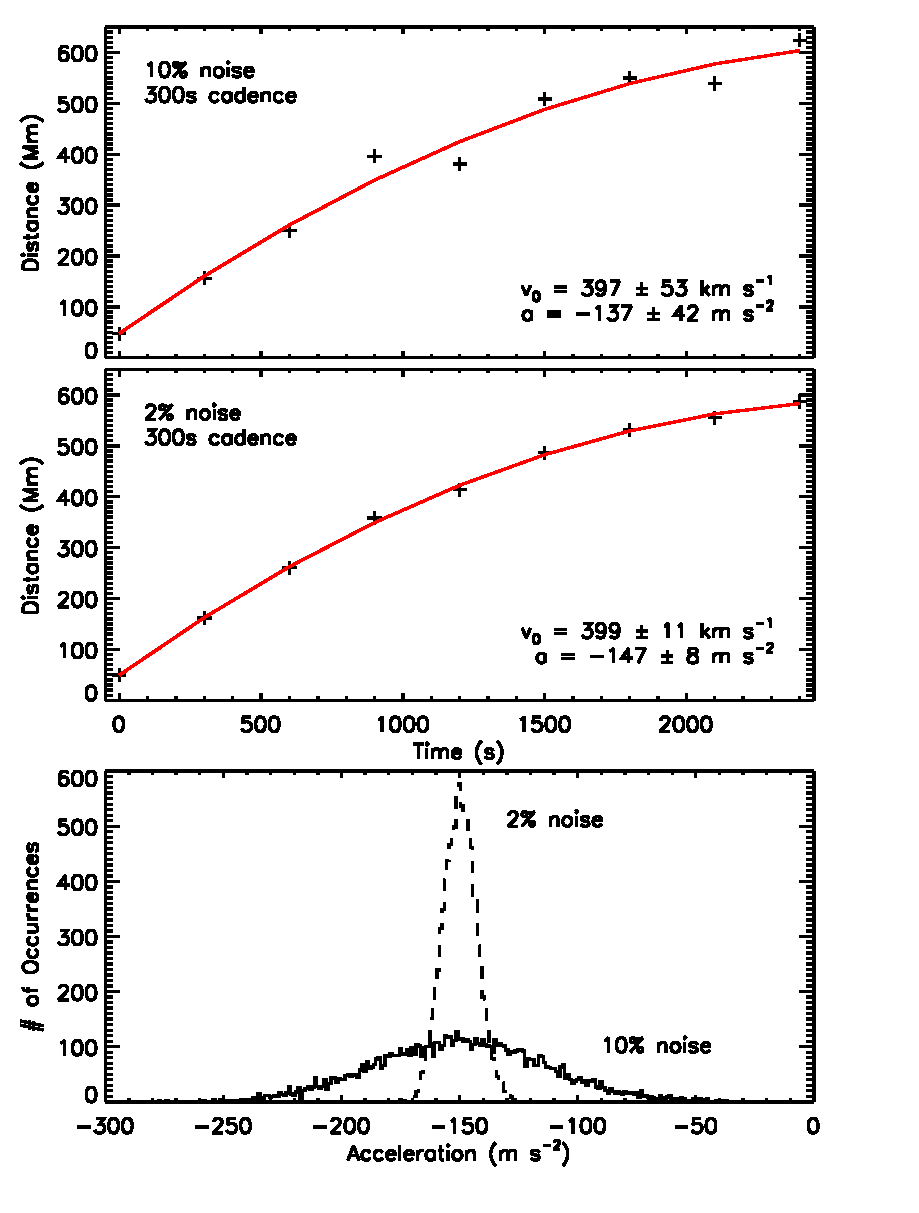
\includegraphics[clip=,trim=0mm 5mm 0mm 0mm,width = 0.45\textwidth]{images/noise_hist_weight.eps}
\caption{Simulated datapoints for noise distributions with 3\,$\sigma$ widths of $\pm$\,10\% (\emph{top}), and $\pm$\,2\% (\emph{middle}) of the model value, at a fixed cadence of 300\,s, and the resulting quadratic fit and $v_0$ and $a$ parameters. The reduced noise level increases the precision in obtaining the true kinematics, as demonstrated by the different distributions of derived accelerations (\emph{bottom}).}
\label{noise_hist_weight}
\end{center}
\end{figure}

\begin{figure}[t]
\begin{center}
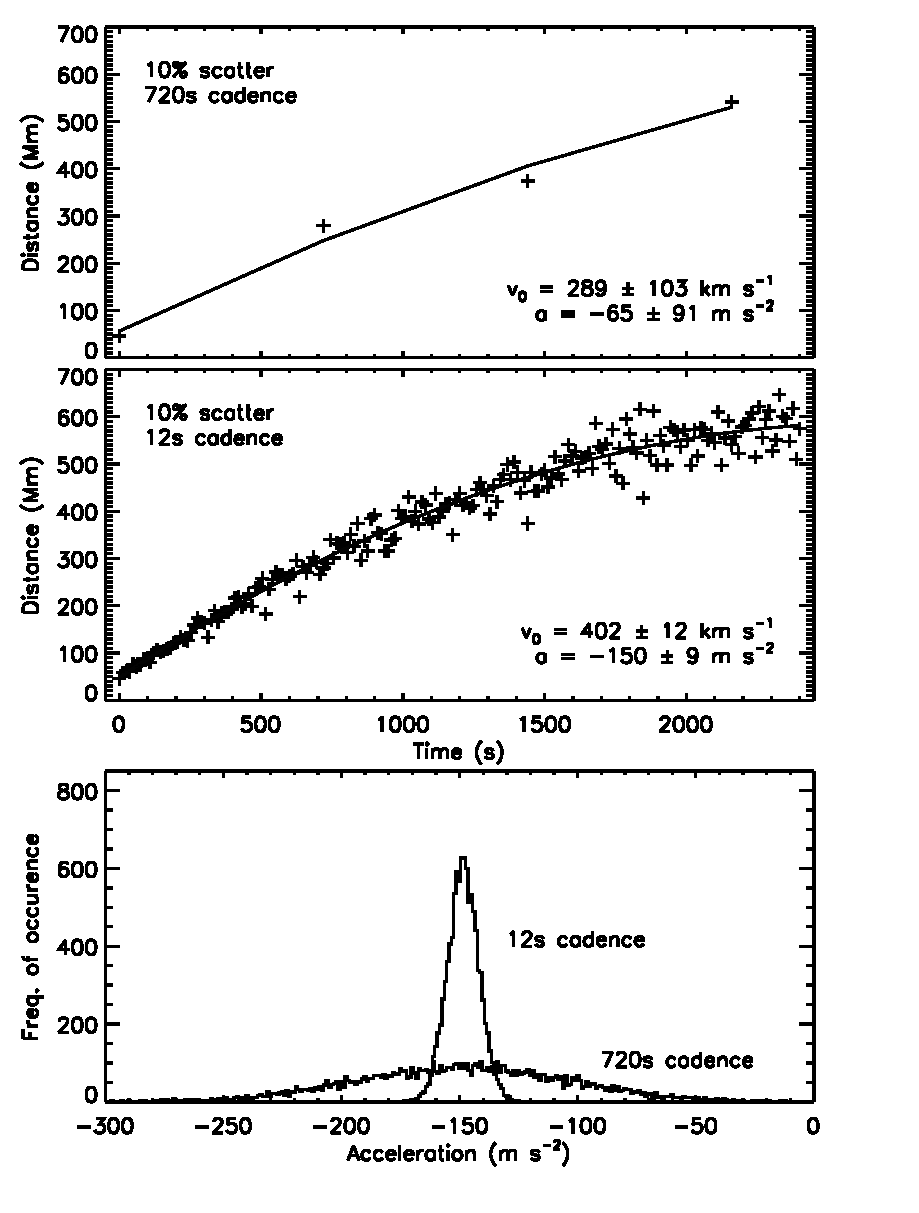
\includegraphics[clip=,trim=0mm 5mm 0mm 0mm,width = 0.45\textwidth]{images/cad_hist_weight.eps}
\caption{Simulated datapoints for sampling cadences of 720\,s (EIT; \emph{top}) and 12\,s (AIA; \emph{middle}), at a fixed noise level of $\pm$\,10\%, and the resulting quadratic fit and $v_0$ and $a$ parameters. The increased cadence offers better precision in obtaining the true kinematics, as demonstrated by the different distributions of derived accelerations (\emph{bottom}).}
\label{cad_hist_weight}
\end{center}
\end{figure}


The effects of varying scatter due to noise on the data of a coronal wave were also examined, demonstrated here for the case of a constant acceleration event. The wave motion is modeled by Equation~\ref{eqn:const_a}, where $r_0$\,=\,50\,Mm is the initial distance of the wave from the source, $v_0$\,=\,400\,km\,s$^{-1}$ is the initial velocity of the wave, and $a$\,=\,$-$150\,m\,s$^{-2}$ is the acceleration of the wave. Figure~\ref{noise_hist_weight} shows the derived kinematics for the simulated dataset with random noise added, shown here for 3\,$\sigma$ limits of 10\,\% (top panel) and 2\,\% (middle panel). A quadratic is then fit to each dataset to test how the noise level affects the precision of the derived kinematics, even in this idealized case of knowing the expected form of the data. The increased noise level acts to smooth out the true kinematics, as demonstrated by the different distributions of derived accelerations (bottom panel).

\subsection{Effect of sampling cadence on deriving kinematics}
\label{subsect:test_lagrange_nonconst}


As an example of the effect of cadence, we first simulate again the constant-acceleration profile of a coronal wave (as in Equation~\ref{eqn:const_a} and Figure~\ref{noise_hist_weight}). The data is sample at cadences akin to the instruments EIT (12\,mins) and AIA (12\,s), at a fixed noise level of 10\,\%. Figure~\ref{cad_hist_weight} shows examples of these, with a quadratic fit to the sample data to test the effect on the derived kinematics. It is clear that the higher-cadence data best resolves the true kinematic profile, providing an accurate estimation of the wave velocity and acceleration. These results are consistent with the observations made by both \citet{2008ApJ...680L..81L} and \citet{2009ApJ...707..503M} and show that the effects of image cadence must be accounted for when trying to derive the true kinematics of a coronal wave.


We next simulate a non-constant acceleration profile for a CME via the following equations (where the constant $x$ is just a scaling factor):
\begin{eqnarray}
h(t)\,=&\,\sqrt{2x}\,t\tan^{-1}\left(\frac{e^{t/2x}}{\sqrt{2x}}\right) \\
v(t)\,=&\,\sqrt{2x}\tan^{-1}\left(\frac{e^{t/2x}}{\sqrt{2x}}\right)+\frac{e^{t/2x}t}{e^{t/x}+2x} \\
a(t)\,=&\,\frac{e^{t/2x}\left(2x\left(t+4x\right)-e^{t/x}\left(t-4x\right)\right)}{2x\left(e^{t/x}+2x\right)^2}
\end{eqnarray}
The acceleration profile exhibits an initial peak followed by a deceleration and then leveling to zero. This is akin to a general impulsive CME that undergoes an initial high-acceleration eruptive phase, and then decelerates to match the solar wind speed during its propagation phase. Thus a model CME height-time profile is generated enabling synthetic observation samples to be taken at different cadences (Figure~\ref{fig_cadence_hva}). 

\begin{figure*}[t]
\centering
\subfigure{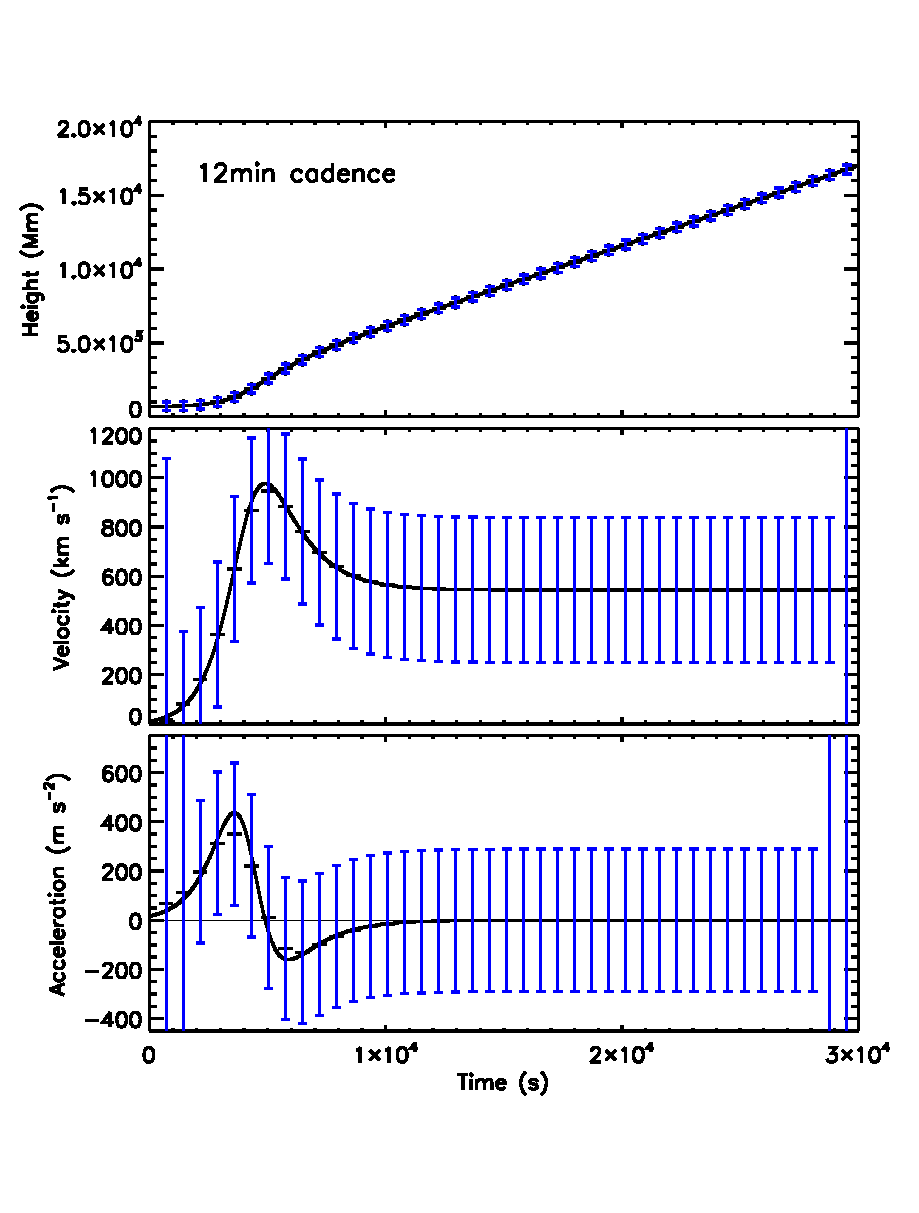
\includegraphics[scale=0.5, trim=0 55 0 50]{images/fig_cadence_hva_12min.eps}}
\subfigure{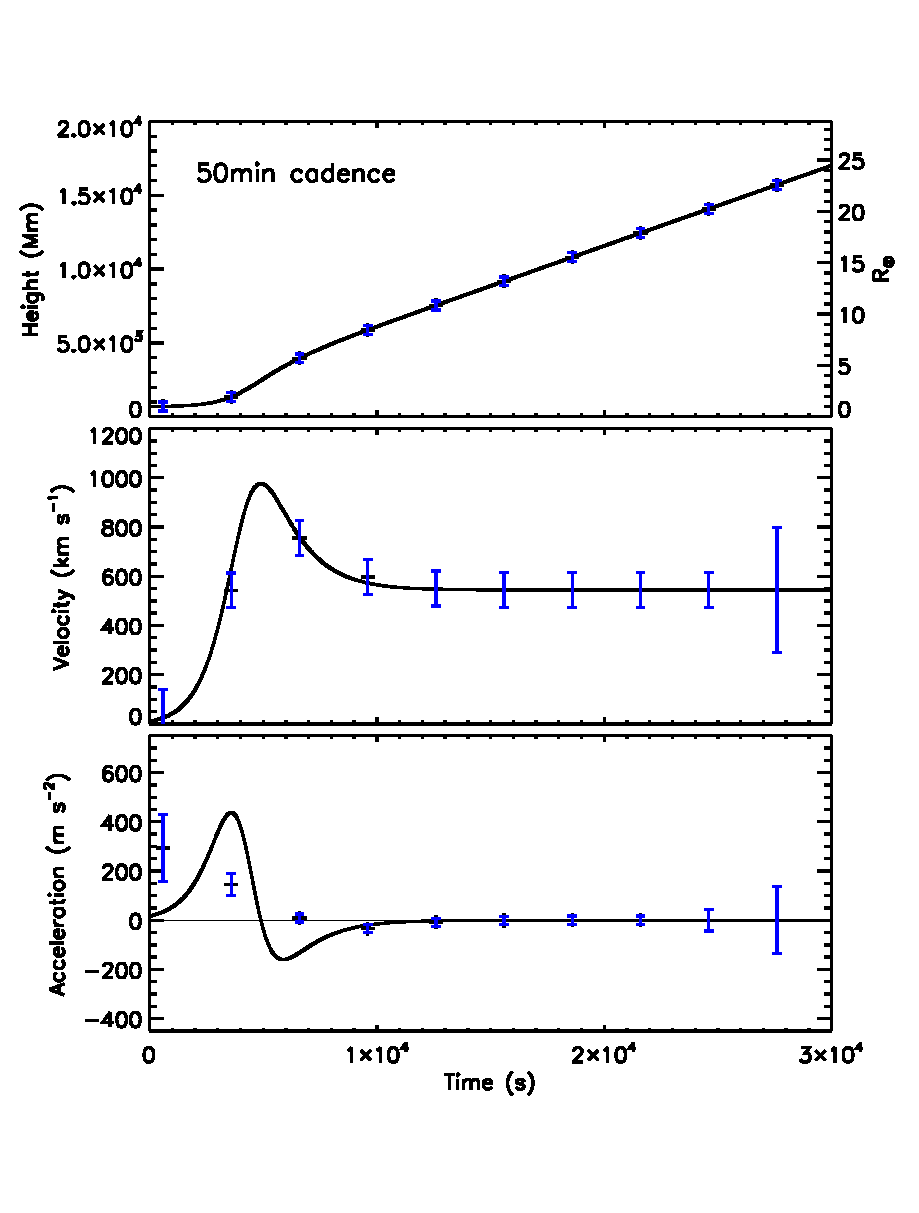
\includegraphics[scale=0.5, trim=0 55 0 50]{images/fig_cadence_hva_50min.eps}}
\subfigure{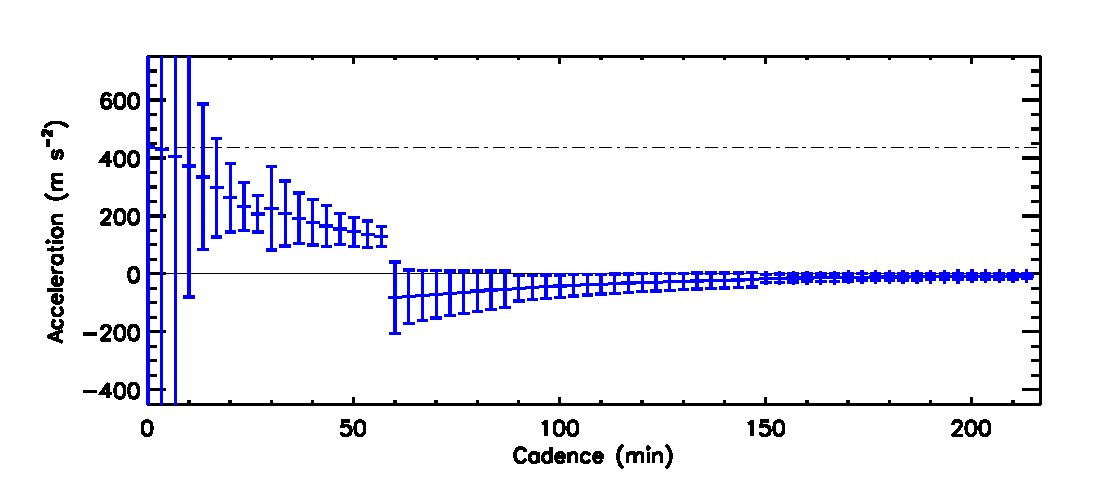
\includegraphics[scale=0.5, trim=0 20 0 25]{images/fig_cadence_1.eps}}
\caption{}
\label{fig_cadence_hva}
\end{figure*}

We investigate the effect of the cadence of the observations on the derivation of the kinematics and associated errorbars using the standard 3-point Lagrangian interpolation. In the first instance fixed 3$\sigma$ errorbars of $\pm$\,300\,Mm are applied to the height-time points, without any noise added. This is useful to simply test the effects of the cadence on the derived velocity and acceleration profiles and their associated errors. The top left and right plots of Figure~\ref{fig_cadence_hva} show the model height-time, velocity and acceleration profiles sampled at cadences of 12 and 50\,mins respectively. As the cadence is reduced, i.e., the cadence time is increased, the errorbars become smaller due to the inverse dependence of the Lagrangian error terms on the time between the datapoints $\Delta t^{-2}$ (see Equation~\ref{vel_err}). However, reducing the cadence reduces the resolution with which the acceleration peak is detectable, and so the acceleration profile is smoothed out. Conversely, the errorbars would become erroneously large for very high-cadence measurements, even though the measurements would better reveal the true trends of the kinematic profiles. This fundamentally implies that the errorbars do not truly reflect the uncertainty on the data at a given cadence, and are in fact completely redundant for these cases.


%As a result, two distinct kinematic forms were simulated here: a quadratic model and a power--law model. Both of these models are typically used to determine the kinematics of these disturbances and have been used extensively in previous work \citep[e.g.,][]{2008ApJ...680L..81L,2008ApJ...681L.113V,2004A&A...418.1101W,2011ApJ...739...89M}. The quadratic model takes the form of Equation~\ref{eqn:const_a} assuming the wave moves with constant acceleration. The power-law fit may be used to identify variable acceleration of the form:
%\begin{equation}
%r(t) = c(t - t_0)^{\gamma}
%\end{equation}
%where $c$ is a constant, $t_0$ is the start time, and $\gamma$ is the exponent.


It is clear therefore, that the variation in both noise and imaging cadence can strongly influence the derived kinematics of a CME or coronal wave, and the 3-point Lagrangian technique does not return useful estimates of the associated uncertainty. However, it is possible to use other techniques along with a bootstrapping approach to overcome these issues, an produce a more statistically sound method for dealing with small datasets such as these. 



\section{Bootstrapping}
\label{sect:simul2}

\begin{figure}[!t]
\begin{center}
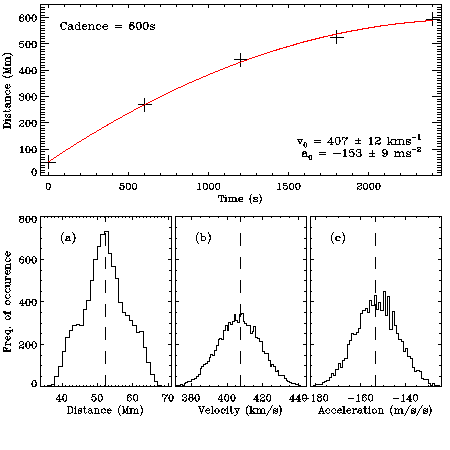
\includegraphics[clip=,trim=0mm 5mm 0mm 0mm,width = 0.49\textwidth]{images/bootstrap.pdf}
\caption{\emph{Top}: Simulated data (asterisks) with bootstrapped fit shown in red and parameters in bottom right. \emph{Bottom}: Histograms showing the distance (a), velocity (b) and acceleration (c) derived using the bootstrapping technique.}
\label{fig:bootstrap}
\end{center}
\end{figure}

When trying to determine an estimator for a particular parameter of interest and subsequently evaluate the accuracy of that estimator, a small sample-size is immediately limiting. So techniques based on resampling methods have been developed, in order to approximate the behavior of the true distribution by resampling the data enough times to generate a maximum likelihood estimator of the distribution. Bootstrapping, first introduced by \citet{Efron:1979p1831} and more recently described in e.g. \citet{1994.book.Efron} and \citet{Chernick1999}, is one such technique, that may be formally defined as follows. Given a random sample of $n$ independent identically distributed vectors $\vec{x} = \left( x_1, x_2, ..., x_n \right)$ from an unknown probability distribution function $\vec{F}$ and a real-valued estimator $\hat{\theta} = s \left( \vec{x} \right)$, a procedure (the bootstrap) to assess the accuracy of $\hat{\theta}$ is defined in terms of the empirical distribution function $\hat{\vec{F}}$, which is the maximum likelihood estimator of the distribution for the observations when no parametric assumptions are made. Otherwise stated, a bootstrap sample $\vec{x}^* = \left( x_1^*, x_2^*, ..., x_n^* \right)$ is generated by randomly sampling with replacement from the population of $n$ objects, giving a resampled version of $\vec{x}$. The bootstrap algorithm then works by drawing many independent bootstrap samples, to estimate the standard error of $\hat{\theta}$ from the observed data $\vec{x}$.

Thus in the cases of CME and coronal wave observations, bootstrap techniques can prove very useful for determining the accuracy of the derived form of their kinematics. The implementation of the bootstrapping technique is as follows:
\begin{enumerate}
\item An initial fit to the data $y$ is obtained, yielding the model fit $\hat{y}$ with parameters $\vec{p}$.
\item The residuals of the fit are calculated: $\epsilon = y - \hat{y}$.
\item The residuals are randomly resampled with replacement to give $\epsilon^*$.
\item The model is then fit to a new data vector $y^* = y + \epsilon^*$ and the parameters $\vec{p}^*$ stored.
\item Steps 3--4 are repeated many times (e.g. 10,000).
\item Confidence intervals on the parameters are determined from the resulting distributions.
\end{enumerate}

 This has the effect of repeating the fit to slightly varying data a large number of times, allowing a distribution of fit values to be obtained. The mean and standard deviation of this distribution then provide the estimated value and associated error of the parameter. This technique is statistically rigorous and produces a more accurate result than a simple model fit to the given data. 

This technique was applied to the simulated data--set used in Section to allow a comparison of the effectiveness of the bootstrapping approach with the numerical differencing techniques. The results of this analysis are shown in Figure~\ref{fig:bootstrap}. The upper panel here shows the simulated data (indicated by the asterisks) with the bootstrapped fit to the data shown by the red line. The kinematics obtained by the bootstrapping approach are given in the bottom right. The bottom panels (a), (b) and (c) show the histograms for the distance, velocity and acceleration parameters respectively. These histograms returned by the bootstrapping approach for each parameter allow a statistical determination of the fit parameters, a fact reflected in the error term for the derived kinematics. 

The kinematics returned by the bootstrapping approach match the model kinematics within one standard deviation, while also producing an accurate estimate with well--defined errors, unlike those of the numerical differencing techniques. It should also be noted that none of the data--points have been removed, unlike the majority of the numerical differencing techniques tested. 

As a result of the simulations carried out to test the different approaches to determining the kinematics of a CBF pulse, the residual resampling bootstrapping technique was chosen as the best method. This fits a model directly to the distance--time measurements, allowing the kinematics of the CBF pulse to be determined to a high degree of accuracy. The kinematics given for each future event studied here therefore reflects the mean value of the bootstrapped distribution, with the associated error given by the standard deviation.

\begin{figure}[t]
\centering
\subfigure{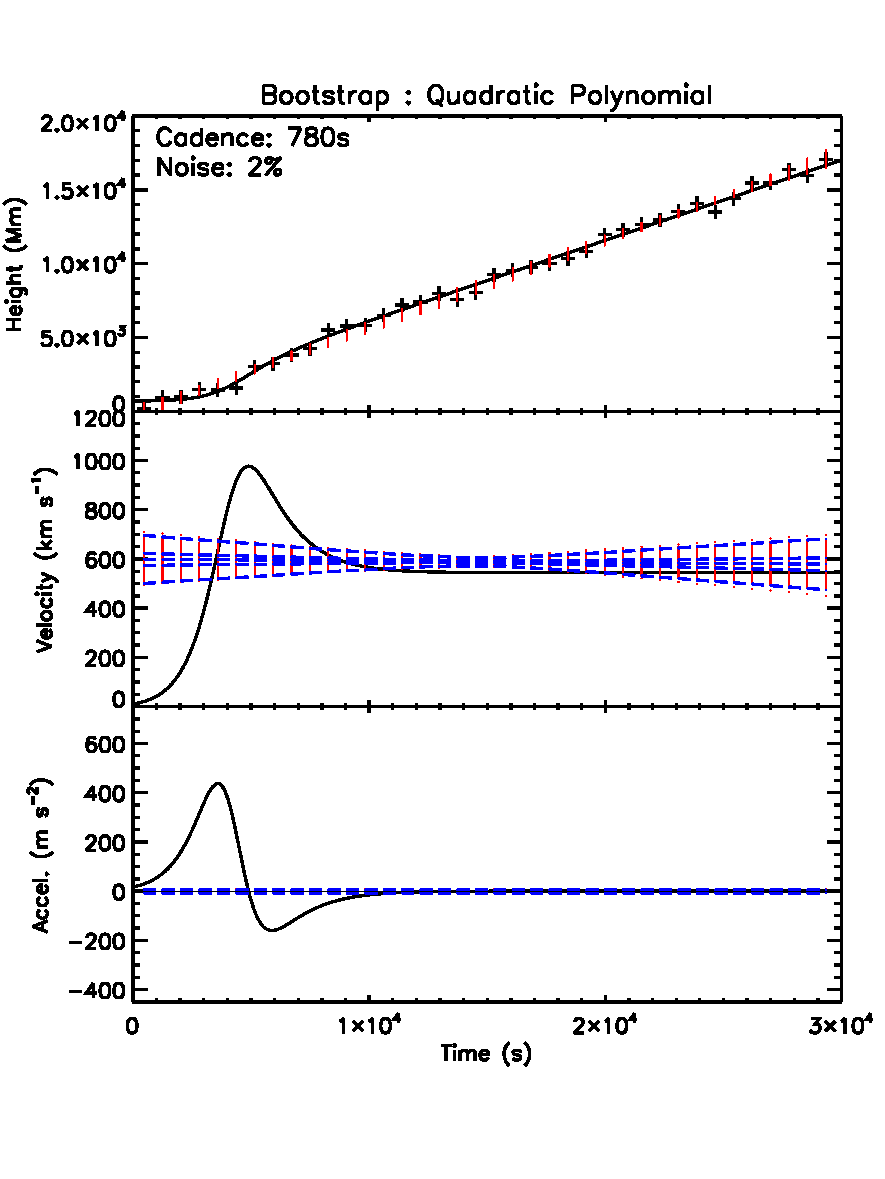
\includegraphics[scale=0.5, trim=0 80 0 30]{images/fig_bootstrap_quadratic.pdf}}
\subfigure{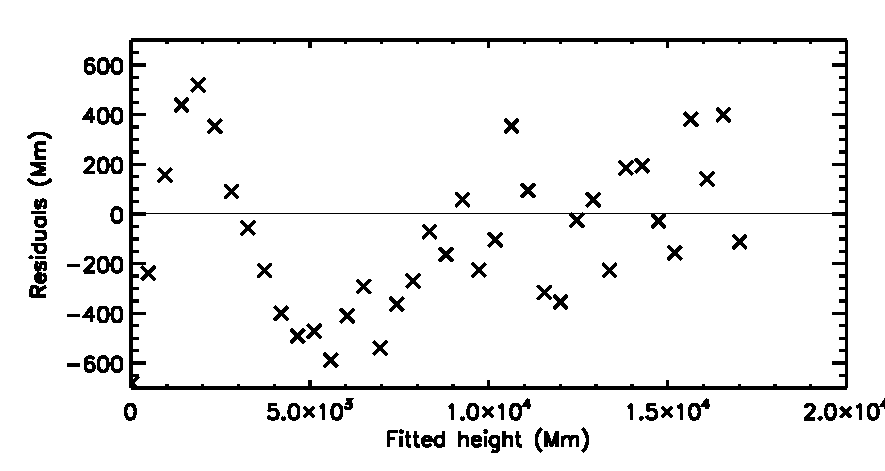
\includegraphics[scale=0.5, trim=0 20 0 0]{images/fig_residuals_quadratic.pdf}}
\caption{}
\label{fig_quadratic}
\end{figure}

\begin{figure}[t]
\centering
\subfigure{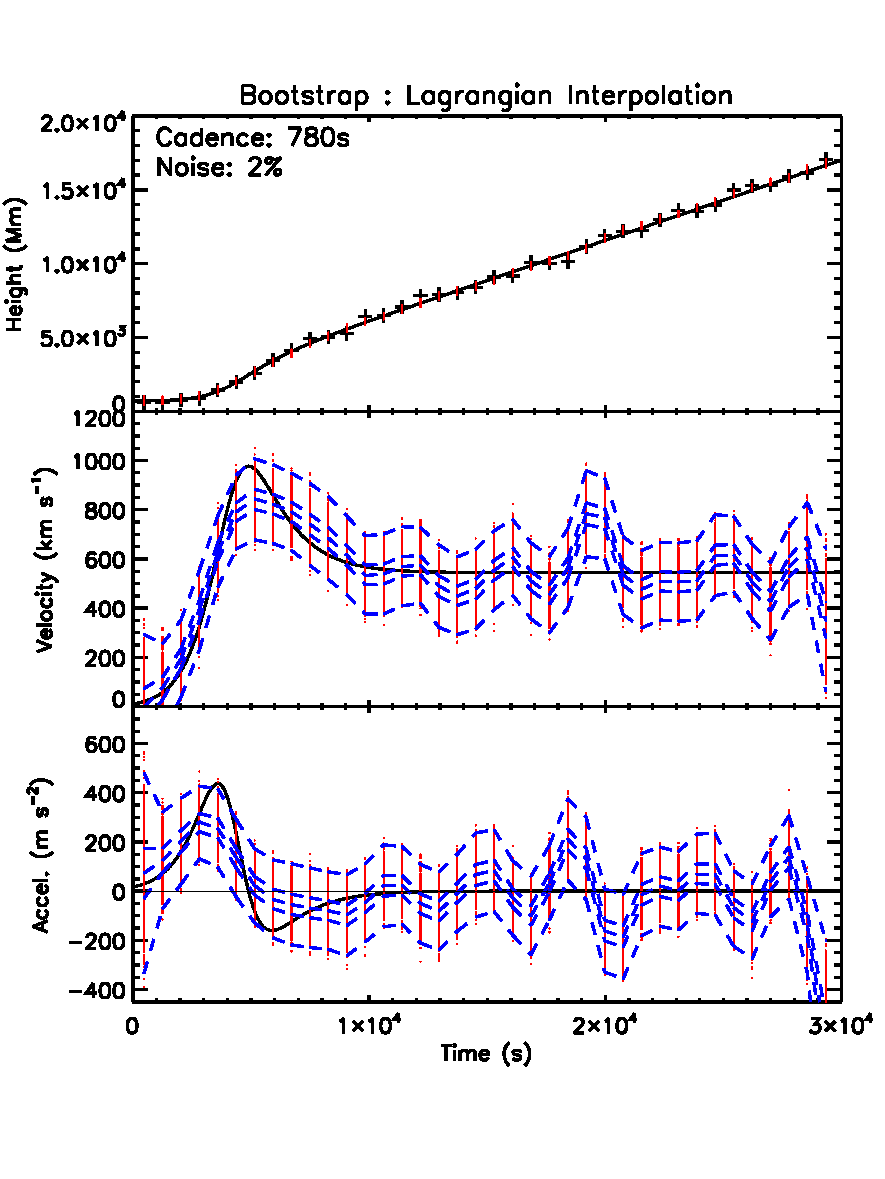
\includegraphics[scale=0.5, trim=0 80 0 30]{images/fig_bootstrap_lagrangian.pdf}}
\subfigure{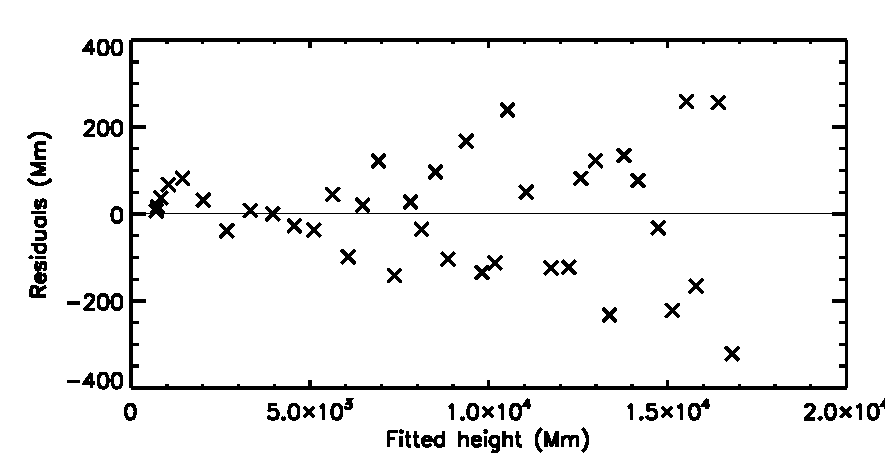
\includegraphics[scale=0.5, trim=0 20 0 0]{images/fig_residuals_lagrangian.pdf}}
\caption{}
\label{fig_lagrangian}
\end{figure}

\begin{figure}[t]
\centering
\subfigure{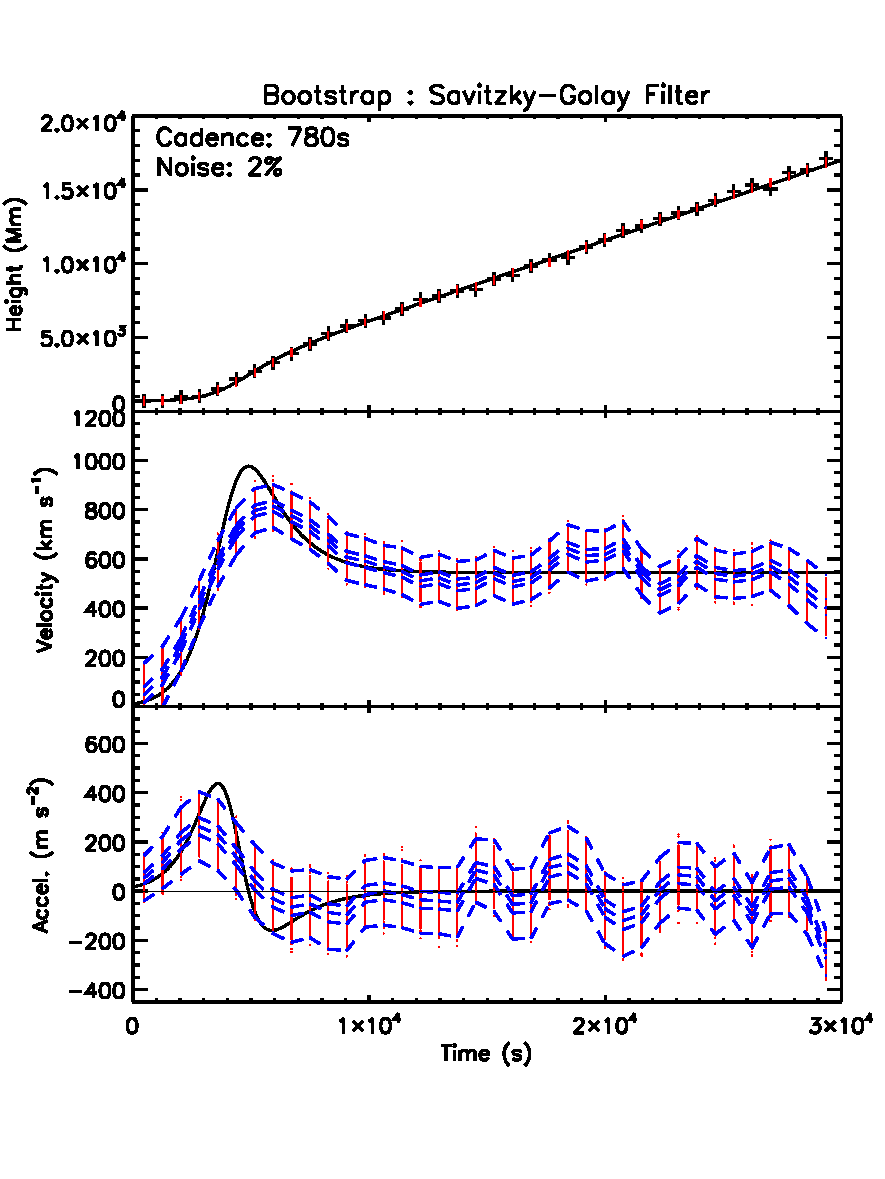
\includegraphics[scale=0.5, trim=0 80 0 30]{images/fig_bootstrap_savgol.pdf}}
\subfigure{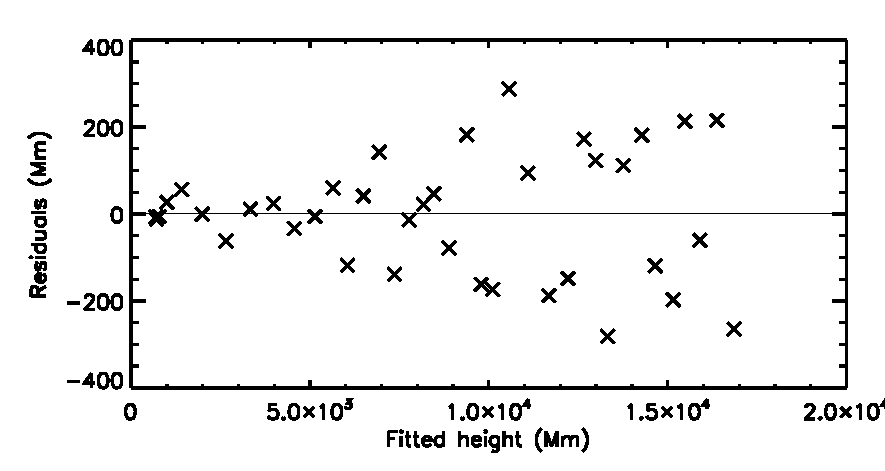
\includegraphics[scale=0.5, trim=0 20 0 0]{images/fig_residuals_savgol.pdf}}
\caption{}
\label{fig_savgol}
\end{figure}


\section{Case Studies}
\label{sect:case_studies}

\subsection{CORIMP}
\label{subsect:corimp}

\subsection{CorPITA}
\label{subsect:corpita}

\section{Conclusions}
\label{sect:conclusions}


\begin{acknowledgements}
This work is supported by SHINE grant 0962716 and NASA grant NNX08AJ07G to the Institute for Astronomy. The SOHO/LASCO data used here are produced by a consortium of the Naval Research Laboratory (USA), Max-Planck-Institut fuer Aeronomie (Germany), Laboratoire d'Astronomie (France), and the University of Birmingham (UK). SOHO is a project of international cooperation between ESA and NASA. The STEREO/SECCHI project is an international consortium of the Naval Research Laboratory (USA), Lockheed Martin Solar and Astrophysics Lab (USA), NASA Goddard Space Flight Center (USA), Rutherford Appleton Laboratory (UK), University of Birmingham (UK), Max-Planck-Institut f\"{u}r Sonnen-systemforschung (Germany), Centre Spatial de Liege (Belgium), Institut d'Optique Th\'{e}orique et Appliqu\'{e}e (France), and Institut d'Astrophysique Spatiale (France). 
\end{acknowledgements}



\bibliographystyle{apj.bst}
\bibliography{references.bib}  



\end{document}